
In the each of the following Exercises, find the coordinates of the focus, axis of the parabola, the equation of the directrix and the length of the latus rectum.
\begin{enumerate}[label=\thesection.\arabic*,ref=\thesection.\theenumi]
\numberwithin{equation}{enumi}
\numberwithin{figure}{enumi}
\numberwithin{table}{enumi}

\item $y^2$=12x 
\label{chapters/11/11/2/1}
\\
\solution
\iffalse
\documentclass[12pt]{article}
\usepackage{graphicx}
\usepackage[none]{hyphenat}
\usepackage{graphicx}
\usepackage{listings}
\usepackage[english]{babel}
\usepackage{graphicx}
\usepackage{caption} 
\usepackage{booktabs}
\usepackage{array}
\usepackage{amssymb} % for \because
\usepackage{amsmath}   % for having text in math mode
\usepackage{extarrows} % for Row operations arrows
\usepackage{listings}
\lstset{
  frame=single,
  breaklines=true
}
\usepackage{hyperref}
  
%Following 2 lines were added to remove the blank page at the beginning
\usepackage{atbegshi}% http://ctan.org/pkg/atbegshi
\AtBeginDocument{\AtBeginShipoutNext{\AtBeginShipoutDiscard}}


%New macro definitions
\newcommand{\mydet}[1]{\ensuremath{\begin{vmatrix}#1\end{vmatrix}}}
\providecommand{\brak}[1]{\ensuremath{\left(#1\right)}}
\providecommand{\norm}[1]{\left\lVert#1\right\rVert}
\providecommand{\abs}[1]{\left\vert#1\right\vert}
\newcommand{\solution}{\noindent \textbf{Solution: }}
\newcommand{\myvec}[1]{\ensuremath{\begin{pmatrix}#1\end{pmatrix}}}
\let\vec\mathbf


\begin{document}

\begin{center}
\title{\textbf{Conic Sections - Parbola}}
\date{\vspace{-5ex}} %Not to print date automatically
\maketitle
\end{center}
\setcounter{page}{1}

\section{11$^{th}$ Maths - Chapter 11}
This is Problem-1 from Exercise 11.2
\begin{enumerate}
\solution 
\fi
The given equation of the parabola can be rearranged as
\begin{align}
    \label{eq:chapters/11/11/2/1/parabolaEq1}
    y^2-12x = 0
\end{align}
The above equation can be equated to the generic equation of conic sections
\begin{align}
	\label{eq:chapters/11/11/2/1/parabolaEq2}
	g\brak{\vec{x}} = \vec{x}^T\vec{V}\vec{x} + 2\vec{u}^T\vec{x} + f = 0 
\end{align}
Comparing coefficients of \eqref{eq:chapters/11/11/2/1/parabolaEq1} and \eqref{eq:chapters/11/11/2/1/parabolaEq2},
\begin{align}
	\label{eq:chapters/11/11/2/1/eqV}
	\vec{V} &= \myvec{ 0 & 0 \\ 0 & 1} \\
	\label{eq:chapters/11/11/2/1/eqU}
	\vec{u} &= -\myvec{6 \\ 0} \\
	\label{eq:chapters/11/11/2/1/eqF}
	f &= 0 
\end{align}
\begin{enumerate}
\item  
From \eqref{eq:chapters/11/11/2/1/eqV}, since $\vec{V}$ is already diagonalized, the Eigen values $\lambda_1$ and $\lambda_2$ are given as 
\begin{align}
	\label{eq:chapters/11/11/2/1/eqEigen1}
	\lambda_1 &= 0 \\
	\label{eq:chapters/11/11/2/1/eqEigen2}
	\lambda_2 &= 1 
\end{align}
and the eigenvector matrix
\begin{align}
	\vec{P} = \vec{I}.
\end{align}
\iffalse
The Eigen vector $\vec{p_1}$ corresponding to Eigen value $\lambda_1$ is computed as shown below
\begin{align}
	\vec{V} &= \myvec{ 0 & 0 \\ 0 & 1} \\
	\label{eq:chapters/11/11/2/1/eqLambda1}
	\vec{V}-\lambda_1\vec{I} &= \myvec{ 0 - \lambda_1 & 0 \\ 0 & 1-\lambda_1} 
\end{align}
Substituting value of $\lambda_1$ from \eqref{eq:chapters/11/11/2/1/eqEigen1} in \eqref{eq:chapters/11/11/2/1/eqLambda1}
\begin{align}
	\eqref{eq:chapters/11/11/2/1/eqLambda1} \implies  \myvec{  0 & 0 \\ 0 & 1}  \\
	\myvec{  0 & 0 \\ 0 & 1}\myvec{x_1 \\ x_2} &= \myvec{0 \\0} 
\end{align}
$x_1$ is free variable and $x_2 = 0$. \\
\fi
\begin{align}
	\therefore 
	%\vec{p_1} &= \myvec{1 \\ 0} \\
	\vec{n} &= \sqrt{\lambda_2}\vec{p_1} \\
%	&= \sqrt{1}\myvec{1 \\ 0} \\
	\label{eq:chapters/11/11/2/1/eqN}
	&= \myvec{1 \\ 0} 
\end{align}
Since
\begin{align}
	\label{eq:chapters/11/11/2/1/eqC}
	c = \frac{\norm{\vec{u}^2}-\lambda_2f}{2\vec{u}^\top\vec{n}},
\end{align}
Substituting values of $\vec{u}, \vec{n}, \lambda_2 \text{ and } f$ in \eqref{eq:chapters/11/11/2/1/eqC}
\begin{align}
	c &= \frac{6^2-1\brak{0}}{-2 \myvec{6 & 0}\myvec{1 \\ 0}} = -3 \\
\end{align}
The focus $\vec{F}$ of parabola is expressed as
\begin{align}
	\vec{F} &= \frac{ce^2\vec{n}-\vec{u}}{\lambda_2} \\
	&= \frac{-3\brak{1}^2\myvec{1 \\0} + \myvec{6 \\ 0}}{1} \\
	&= \myvec{3 \\ 0}
\end{align}
\item The directrix is given by
\begin{align}
	\vec{n}^\top\vec{x} &= c \\
	\label{eq:chapters/11/11/2/1/eqDir}
\implies	\myvec{1 & 0}\vec{x} &= -3
\end{align}

\item The equation for the axis of parabola passing through $\vec{F}$ and orthogonal to the directrix is given as  
\begin{align}
	\label{eq:chapters/11/11/2/1/eqAxis}
	\vec{m}^\top\brak{\vec{x}-\vec{F}} &= 0
\end{align}
where $\vec{m}$ is the normal vector to the axis and also the slope of the directrix.
\begin{align}
	\because \vec{n} = \myvec{1 \\ 0 }, \vec{m} &= \myvec{0 \\ 1} \\
	\eqref{eq:chapters/11/11/2/1/eqAxis} \implies \myvec{0 & 1}\myvec{\vec{x} - \myvec{3 \\ 0}} &= 0\\
	\text{or, }	\myvec{0 & 1}\vec{x} &= 0 
\end{align}
\item The latus rectum of a parabola is given by 
\begin{align}
	l &= \frac{\eta}{\lambda_2}  
	 = \frac{2\vec{u}^\top\vec{p_1}}{\lambda_2} \\
	 &= \frac{2\myvec{6 & 0}\myvec{1 \\ 0}}{1} \\
	 &= 12 \text{ units }
\end{align}
The relevant diagram is shown in Fig. \ref{fig:11/11/2/1Fig1}
\begin{figure}[!h]
	\begin{center}
		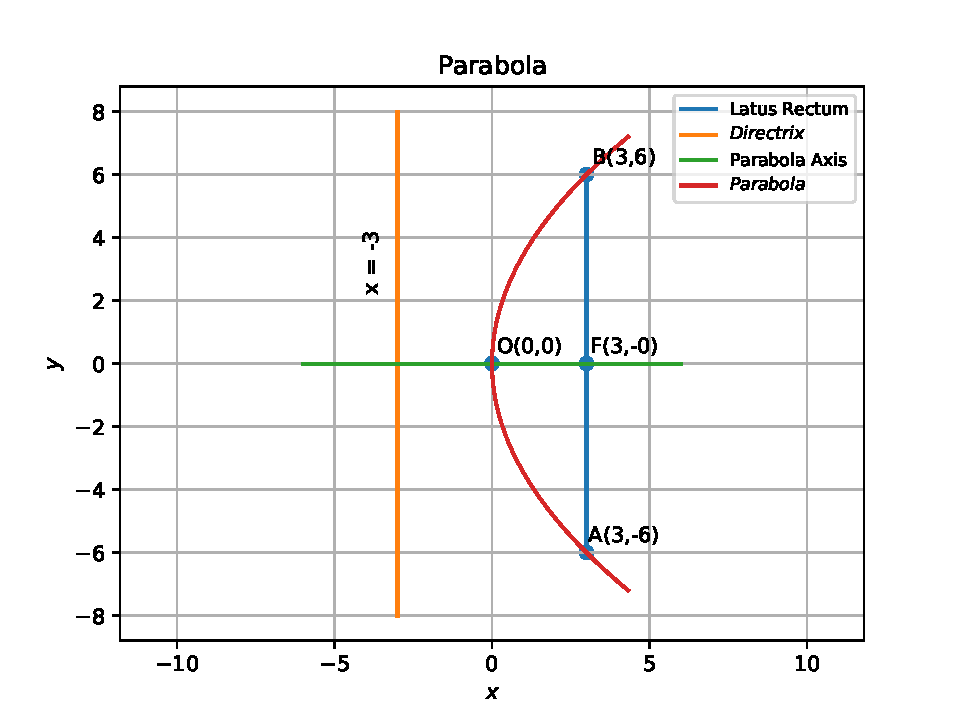
\includegraphics[width=\columnwidth]{chapters/11/11/2/1/figs/problem1.pdf}
	\end{center}
\caption{}
\label{fig:11/11/2/1Fig1}
\end{figure}
\end{enumerate}



\item $x^2$=6y 
\\
\solution
\iffalse
\documentclass[12pt]{article}
\usepackage{graphicx}
\usepackage{amsmath}
\usepackage{mathtools}
\usepackage{gensymb}

\newcommand{\mydet}[1]{\ensuremath{\begin{vmatrix}#1\end{vmatrix}}}
\providecommand{\brak}[1]{\ensuremath{\left(#1\right)}}
\providecommand{\norm}[1]{\left\lVert#1\right\rVert}
\newcommand{\solution}{\noindent \textbf{Solution: }}
\newcommand{\myvec}[1]{\ensuremath{\begin{pmatrix}#1\end{pmatrix}}}
\let\vec\mathbf

\begin{document}
\begin{center}
\textbf\large{CONIC SECTIONS}

\end{center}
\section*{Excercise 11.2}

Q2.Find the coordinates of the focus, axis of the parabola, the equation of the directrix and the length of the latus rectum of a parabola whose equation is given by $x^2=6y$.

\solution
\fi
The given equation of the parabola can be rearranged as
\begin{align}
	\label{eq:chapters/11/11/2/2/parabolaEq1}
	x^2-6y=0
\end{align}
The above equation can be equated to the generic equation of conic sections
\begin{align}
	\label{eq:chapters/11/11/2/2/parabolaEq2}
	g\brak{\vec{x}}=\vec{x}^\top \vec{V}\vec{x}+2\vec{u}^\top \vec{x}+f=0
\end{align}
Comparing the coefficients of both equations \eqref{eq:chapters/11/11/2/2/parabolaEq1} and \eqref{eq:chapters/11/11/2/2/parabolaEq2}
\begin{align}
	\label{eq:chapters/11/11/2/2/eqV}
	\vec{V} &= \myvec{1&0\\0&0}\\
	\label{eq:chapters/11/11/2/2/eqU}
	\vec{u} &= -\myvec{0\\3}\\
	\label{eq:chapters/11/11/2/2/eqF}
	f &= 0
\end{align}
\begin{enumerate}
\item From equation \eqref{eq:chapters/11/11/2/2/eqV}, since $\vec{V}$ is already diagonalized, the Eigen values $\lambda_1 \text{ and } \lambda_2$ are given as
\begin{align}
	\label{eq:chapters/11/11/2/2/eqEigen1}
	\lambda_1 &= 1\\
	\label{eq:chapters/11/11/2/2/eqEigen2}
	\lambda_2 &= 0
\end{align}
And the corresponding eigen vector matrix $\vec{P}$ is indentity, so the Eigen vector $\vec{p}_2$ corresponding to Eigen value $\lambda_2$ is
\begin{align}
	\vec{p}_2 &= \myvec{0\\1}\\
	\vec{n} &= \sqrt{\lambda_1}\vec{p}_2\\
		&= \sqrt{1}\myvec{0\\1}\\
		&= \myvec{0\\1}
\end{align}
Now,
\begin{align}
	\label{eq:chapters/11/11/2/2/eqC}
	c = \frac{\norm{\vec{u}}^2 - \lambda_1 f}{2\vec{u}^\top \vec{n}}
\end{align}
Substituting values of $\vec{u},\vec{n},\lambda_1 \text{ and } f$ in \eqref{eq:chapters/11/11/2/2/eqC}
\begin{align}
	c = \frac{3^2-1\brak{0}}{-2\myvec{0&3}\myvec{0\\1}} = -\frac{3}{2}
\end{align}
The focus $\vec{F}$ of parabola is expressed as
\begin{align}
	\vec{F} &= \frac{ce^2 \vec{n}-\vec{u}}{\lambda_1}\\
		&= \frac{-\frac{3}{2}\brak{1}^2 \myvec{0\\1}+\myvec{0\\3}}{1}\\
		&= \myvec{0\\\frac{3}{2}}
\end{align}
\item Equation of directrix is given as
\begin{align}
	\vec{n}^\top \vec{x} &= c\\
	\myvec{0&1}\vec{x} &= -\frac{3}{2}
\end{align}
\item The equation for the axis of parabola passing through $\vec{F}$ and orthogonal to the directrix is given as
\begin{align}
	\label{eq:chapters/11/11/2/2/eqM}
	\vec{m}^\top \brak{\vec{x}-\vec{F}} = 0
\end{align}
where $\vec{m}$ is the normal vector to the axis and also the slope of the directrix. Now since
\begin{align}
	\vec{n} = \myvec{0\\1}\\
	\vec{m} = \myvec{1\\0}
\end{align}
Substituting in \eqref{eq:chapters/11/11/2/2/eqM}
\begin{align}
	\myvec{1&0}\myvec{\vec{x}-\myvec{0\\\frac{3}{2}}}&=0\\
	\myvec{1&0}\vec{x} &= 0
\end{align}
\item The latus rectum of a parabola is given by
\begin{align}
	l&=\frac{\eta}{\lambda_1}\\
	 &=\frac{2\vec{u}^\top \vec{p}_2}{\lambda_1}\\
	 &=\frac{2\myvec{0&3}\myvec{0\\1}}{1}\\
	 &=6 \text{ units }
\end{align}
See Fig. \ref{fig:chapters/11/11/2/2/Fig1}
\begin{figure}[!h]
	\begin{center} 
	    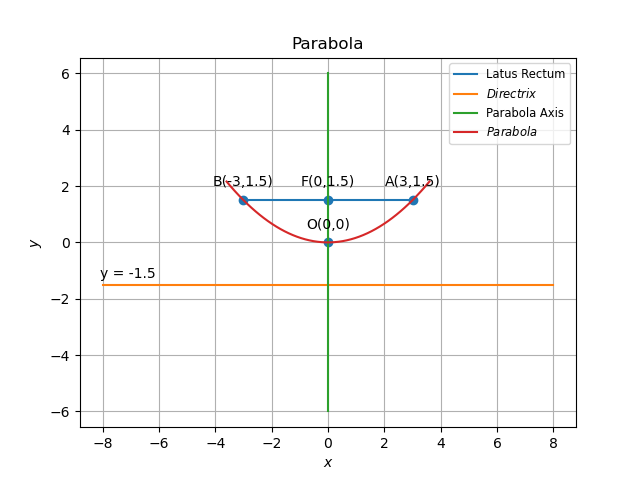
\includegraphics[width=\columnwidth]{chapters/11/11/2/2/figs/parabola}
	\end{center}
\caption{}
\label{fig:chapters/11/11/2/2/Fig1}
\end{figure}
\end{enumerate}





\item Find the coordinates of the focus, axis of the
parabola, the equation of the directrix and the length of the latus rectum of $y^2 = –8x$
\\
\solution
\iffalse
\documentclass[journal,12pt,twocolumn]{IEEEtran}
\usepackage{setspace}
\usepackage{gensymb}
\singlespacing
\usepackage[cmex10]{amsmath}
\usepackage{amsthm}
\usepackage{mathrsfs}
\usepackage{txfonts}
\usepackage{stfloats}
\usepackage{bm}
\usepackage{cite}
\usepackage{cases}
\usepackage{subfig}
\usepackage{longtable}
\usepackage{multirow}
\usepackage{enumitem}
\usepackage{mathtools}
\usepackage{steinmetz}
\usepackage{tikz}
\usepackage{circuitikz}
\usepackage{verbatim}
\usepackage{tfrupee}
\usepackage[breaklinks=true]{hyperref}
\usepackage{tkz-euclide}
\usetikzlibrary{calc,math}
\usepackage{listings}
    \usepackage{color}                                            %%
    \usepackage{array}                                            %%
    \usepackage{longtable}                                        %%
    \usepackage{calc}                                             %%
    \usepackage{multirow}                                         %%
    \usepackage{hhline}                                           %%
    \usepackage{ifthen}                                           %%
  %optionally (for landscape tables embedded in another document): %%
    \usepackage{lscape}     
\usepackage{multicol}
\usepackage{chngcntr}
\DeclareMathOperator*{\Res}{Res}
\renewcommand\thesection{\arabic{section}}
\renewcommand\thesubsection{\thesection.\arabic{subsection}}
\renewcommand\thesubsubsection{\thesubsection.\arabic{subsubsection}}

\renewcommand\thesectiondis{\arabic{section}}
\renewcommand\thesubsectiondis{\thesectiondis.\arabic{subsection}}
\renewcommand\thesubsubsectiondis{\thesubsectiondis.\arabic{subsubsection}}

% correct bad hyphenation here
\hyphenation{op-tical net-works semi-conduc-tor}
\def\inputGnumericTable{}                                 %%

\lstset{
frame=single, 
breaklines=true,
columns=fullflexible
}

\begin{document}


\newtheorem{theorem}{Theorem}[section]
\newtheorem{problem}{Problem}
\newtheorem{proposition}{Proposition}[section]
\newtheorem{lemma}{Lemma}[section]
\newtheorem{corollary}[theorem]{Corollary}
\newtheorem{example}{Example}[section]
\newtheorem{definition}[problem]{Definition}
\newcommand{\BEQA}{\begin{eqnarray}}
\newcommand{\EEQA}{\end{eqnarray}}
\newcommand{\define}{\stackrel{\triangle}{=}}

\bibliographystyle{IEEEtran}
\providecommand{\mbf}{\mathbf}
\providecommand{\pr}[1]{\ensuremath{\Pr\left(#1\right)}}
\providecommand{\qfunc}[1]{\ensuremath{Q\left(#1\right)}}
\providecommand{\sbrak}[1]{\ensuremath{{}\left[#1\right]}}
\providecommand{\lsbrak}[1]{\ensuremath{{}\left[#1\right.}}
\providecommand{\rsbrak}[1]{\ensuremath{{}\left.#1\right]}}
\providecommand{\brak}[1]{\ensuremath{\left(#1\right)}}
\providecommand{\lbrak}[1]{\ensuremath{\left(#1\right.}}
\providecommand{\rbrak}[1]{\ensuremath{\left.#1\right)}}
\providecommand{\cbrak}[1]{\ensuremath{\left\{#1\right\}}}
\providecommand{\lcbrak}[1]{\ensuremath{\left\{#1\right.}}
\providecommand{\rcbrak}[1]{\ensuremath{\left.#1\right\}}}
\theoremstyle{remark}
\newtheorem{rem}{Remark}
\newcommand{\sgn}{\mathop{\mathrm{sgn}}}
\providecommand{\abs}[1]{\left\vert#1\right\vert}
\providecommand{\res}[1]{\Res\displaylimits_{#1}} 
\providecommand{\norm}[1]{\left\lVert#1\right\rVert}
\providecommand{\mtx}[1]{\mathbf{#1}}
\providecommand{\mean}[1]{E\left[ #1 \right]}
\providecommand{\fourier}{\overset{\mathcal{F}}{ \rightleftharpoons}}
\providecommand{\system}{\overset{\mathcal{H}}{ \longleftrightarrow}}
\newcommand{\solution}{\noindent \textbf{Solution: }}
\newcommand{\cosec}{\,\text{cosec}\,}
\providecommand{\dec}[2]{\ensuremath{\overset{#1}{\underset{#2}{\gtrless}}}}
\newcommand{\myvec}[1]{\ensuremath{\begin{pmatrix}#1\end{pmatrix}}}
\newcommand{\mydet}[1]{\ensuremath{\begin{vmatrix}#1\end{vmatrix}}}
\numberwithin{equation}{subsection}
\makeatletter
\@addtoreset{figure}{problem}
\makeatother

\let\StandardTheFigure\thefigure
\let\vec\mathbf
\renewcommand{\thefigure}{\theproblem}



\def\putbox#1#2#3{\makebox[0in][l]{\makebox[#1][l]{}\raisebox{\baselineskip}[0in][0in]{\raisebox{#2}[0in][0in]{#3}}}}
     \def\rightbox#1{\makebox[0in][r]{#1}}
     \def\centbox#1{\makebox[0in]{#1}}
     \def\topbox#1{\raisebox{-\baselineskip}[0in][0in]{#1}}
     \def\midbox#1{\raisebox{-0.5\baselineskip}[0in][0in]{#1}}

\vspace{3cm}


\title{Assignment 1}
\author{Jaswanth Chowdary Madala}





% make the title area
\maketitle

\newpage

%\tableofcontents

\bigskip

\renewcommand{\thefigure}{\theenumi}
\renewcommand{\thetable}{\theenumi}


\begin{enumerate}

\textbf{Solution:}
\fi
The given equation of the parabola can be rearranged as
\begin{align}
y^2+8x = 0
\label{eq:chapters/11/11/2/3/1}
\end{align}
The above equation can be equated to the generic equation of conic sections
\begin{align}
\text{g}\brak{\vec{x}} = \vec{x}^T\vec{V}\vec{x} + 2\vec{u}^T\vec{x} + f = 0
\label{eq:chapters/11/11/2/3/2} 
\end{align}
Comparing coefficients of \eqref{eq:chapters/11/11/2/3/1} and \eqref{eq:chapters/11/11/2/3/2}, we get the parameters as given in Table \ref{tab:chapters/11/11/2/3/1}
\begin{table}[h]
\centering
%%%%%%%%%%%%%%%%%%%%%%%%%%%%%%%%%%%%%%%%%%%%%%%%%%%%%%%%%%%%%%%%%%%%%%
%%                                                                  %%
%%  This is a LaTeX2e table fragment exported from Gnumeric.        %%
%%                                                                  %%
%%%%%%%%%%%%%%%%%%%%%%%%%%%%%%%%%%%%%%%%%%%%%%%%%%%%%%%%%%%%%%%%%%%%%%

\begin{center}
\begin{tabular}{|c|c|}
\hline
\textbf{Parameter}& \textbf{Value}\\ \hline
$\vec{V}$		 &	$\myvec{0&0\\0&1}$\\ \hline
$\vec{u}$		 &	$\myvec{4\\0}$\\ \hline
$f$				 &  0 \\ \hline
\end{tabular}
\end{center}

\caption{}
\label{tab:chapters/11/11/2/3/1}
\end{table}
\begin{enumerate}
\item Focus: Since $\vec{V}$ is already diagonalized, the Eigen values $\lambda_1$ and $\lambda_2$ are given as 
\begin{align}
\lambda_1 = 0,\,
\lambda_2 = 1 
\end{align}
and the eigenvector matrix
\begin{align}
	\vec{P} = \vec{I} \implies 
\vec{p_1} &= \myvec{1 \\ 0} \\
	\text{and }\vec{n} &= \sqrt{\lambda_2}\vec{p_1} 
= \myvec{1 \\ 0} 
\end{align}
%
Since
\begin{align}
\label{eq:chapters/11/11/2/3/3}
c = \frac{\norm{\vec{u}^2}-\lambda_2f}{2\vec{u}^\top\vec{n}},
\end{align}
Substituting values of $\vec{u}, \vec{n}, \lambda_2 \text{ and } f$ in \eqref{eq:chapters/11/11/2/3/3}, we get
\begin{align}
c &= \frac{4^2-1\brak{0}}{2 \myvec{4 & 0}\myvec{1 \\ 0}} = 2
\end{align}
The focus $\vec{F}$ of parabola is expressed as
\begin{align}
\vec{F} &= \frac{ce^2\vec{n}-\vec{u}}{\lambda_2} 
= \myvec{-2 \\ 0}
\end{align}
\item Directrix: The directrix is given by
\begin{align}
\vec{n}^\top\vec{x} &= c \\
\implies	\myvec{1 & 0}\vec{x} &= 2
\end{align}
%
\item Axis: The equation for the axis of parabola, passing through $\vec{F}$ and orthogonal to the directrix is given as  
\begin{align}
\vec{m}^\top\brak{\vec{x}-\vec{F}} &= 0
\label{eq:chapters/11/11/2/3/4}
\end{align}
where $\vec{m}$ is the normal vector to the axis and also the slope of the directrix. Since
\begin{align}
	\vec{n} = \myvec{1 \\ 0 },\,
	\vec{m} &= \myvec{0 \\ 1} \\
\end{align}
the axis is given by
\begin{align}
\myvec{0 & 1}\myvec{\vec{x} - \myvec{-2 \\ 0}} &= 0\\
\implies \myvec{0 & 1}\vec{x} &= 0 
\end{align}
\item Latus rectum: The latus rectum of a parabola is given by 
\begin{align}
	l &= \frac{\eta}{\lambda_2}  
	 = \frac{2\vec{u}^\top\vec{p_1}}{\lambda_2} \\
	 &= 8 \text{ units }
\end{align}
\end{enumerate}
See Fig. 
\ref{fig:chapters/11/11/2/3/1}.
\begin{figure}[ht]
\centering
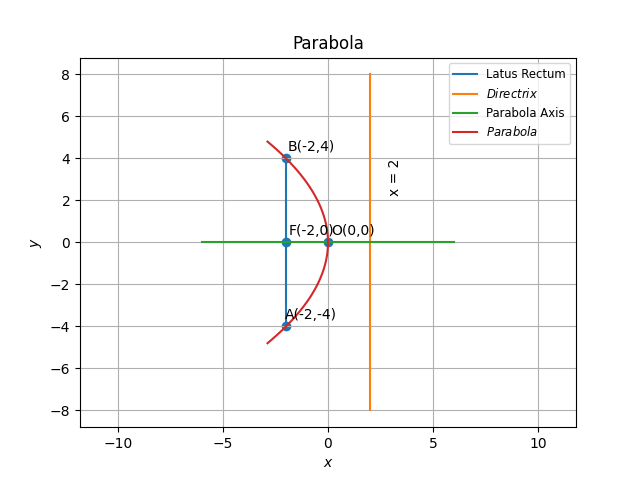
\includegraphics[width = \columnwidth]{chapters/11/11/2/3/figs/fig.png}
\caption{Graph}
\label{fig:chapters/11/11/2/3/1}
\end{figure}

\item $y^2$=-8x

\item $x^2$=-16y
\\
\solution
\iffalse
\documentclass[12pt]{article}
\usepackage{graphicx}
\usepackage{amsmath}
\usepackage{mathtools}
\usepackage{gensymb}

\newcommand{\mydet}[1]{\ensuremath{\begin{vmatrix}#1\end{vmatrix}}}
\providecommand{\brak}[1]{\ensuremath{\left(#1\right)}}
\providecommand{\norm}[1]{\left\lVert#1\right\rVert}
\newcommand{\solution}{\noindent \textbf{Solution: }}
\newcommand{\myvec}[1]{\ensuremath{\begin{pmatrix}#1\end{pmatrix}}}
\let\vec\mathbf

\begin{document}
\begin{center}
\textbf\large{CONIC SECTIONS}

\end{center}
\section*{Excercise 11.2.4}
	Find the coordinates of the focus, axis of the parabola, the equation of the directrix and the length of the latus rectum of a parabola whose equation is given by $x^2=-16y$.\\

\solution
\fi
The given equation of the parabola can be written as
\begin{align}
	\label{eq:chapters/11/11/2/4/parabolaEq1}
	x^2+16y=0
\end{align}
The general equation for conic section is
\begin{align}
	\label{eq:chapters/11/11/2/4/parabolaEq2}
	g\brak{\vec{x}}=\vec{x}^\top \vec{V}\vec{x}+2\vec{u}^\top \vec{x}+f=0
\end{align}
Comparaing both equations \eqref{eq:chapters/11/11/2/4/parabolaEq1} and \eqref{eq:chapters/11/11/2/4/parabolaEq2} we get,
\begin{align}
	\label{eq:chapters/11/11/2/4/eqV}
	\vec{V} &= \myvec{1&0\\0&0}\\
	\label{eq:chapters/11/11/2/4/eqU}
	\vec{u} &= \myvec{0\\8}\\
	\label{eq:chapters/11/11/2/4/eqF}
	f &= 0
\end{align}
\begin{enumerate}
\item As   $\vec{V}$ matrix is already diagonalized \eqref{eq:chapters/11/11/2/4/eqV}, the Eigen values $\lambda_1 \text{ and } \lambda_2$ are given as
\begin{align}
	\label{eq:chapters/11/11/2/4/eqEigen1}
	\lambda_1 &= 1\\
	\label{eq:chapters/11/11/2/4/eqEigen2}
	\lambda_2 &= 0
\end{align}
Eigen vector matrix $\vec{P}$ is identical the eigen vector $\vec{P}_2$ by eigen value $\lambda_2$ is 
\begin{align}
	\vec{p}_2 &= \myvec{0\\1}\\
	\vec{n} &= \sqrt{\lambda_1}\vec{p}_2\\
		&= \sqrt{1}\myvec{0\\1}\\
		&= \myvec{0\\1}
\end{align}
So,
\begin{align}
	\label{eq:chapters/11/11/2/4/eqC}
	 \frac{\norm{\vec{u}}^2 - \lambda_1 f}{2\vec{u}^\top \vec{n}}&= c
\end{align}
Substituting  $\vec{u},\vec{n},\lambda_1 \text{ and } f$ values in \eqref{eq:chapters/11/11/2/4/eqC} we get 
\begin{align}
	c = \frac{8^2-1\brak{0}}{2\myvec{0&8}\myvec{0\\1}} = 4
\end{align}
The focus $\vec{F}$ of parabola is 
\begin{align}
	\vec{F} &= \frac{ce^2 \vec{n}-\vec{u}}{\lambda_1}\\
		&= \frac{4\brak{1}^2 \myvec{0\\1}-\myvec{0\\8}}{1}\\
		&= \myvec{0\\-4}
\end{align}
\item Equation of directrix is given as
\begin{align}
	\vec{n}^\top \vec{x} &= c\\
	\myvec{0&1}\vec{x} &= 4\\
	\vec{x}&= 4
\end{align}
\item Equation for tha axis of parabola is 
\begin{align}
	\vec{m}^\top \brak{\vec{x}-\vec{F}} = 0\label{20}
\end{align}
where $\vec{m}$ is the normal vector to the axis and also the slope of the directrix
\begin{align}
	\vec{n} = \myvec{0\\1}\\
	\vec{m} = \myvec{1\\0}
\end{align}
Substituting in \eqref{20}
\begin{align}
	\myvec{1&0}\myvec{\vec{x}-\myvec{0\\-4}}&=0\\
	\myvec{1&0}\vec{x} &= 0\\
	\vec{x}=0
\end{align}
\item Latus rectum of  parabola is 
\begin{align}
	l&=\frac{\eta}{\lambda_1}\\
	 &=\frac{2\vec{u}^\top \vec{p}_2}{\lambda_1}\\
	 &=\frac{2\myvec{0&8}\myvec{0\\1}}{1}\\
	 &=16 \text{ units }
\end{align}
\begin{figure}[!h]
	\begin{center} 
	    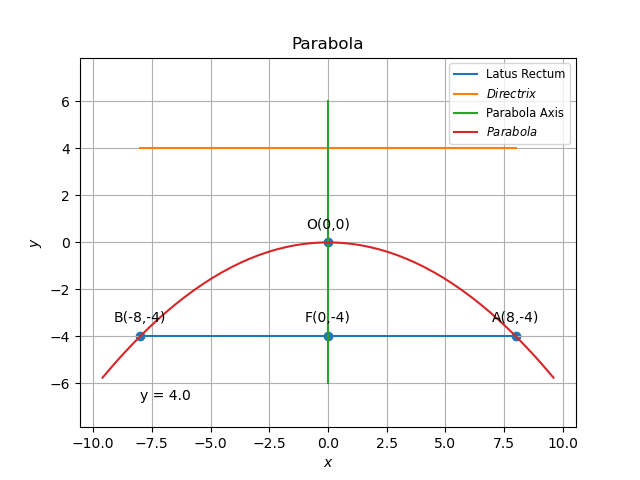
\includegraphics[width=\columnwidth]{chapters/11/11/2/4/figs/parabola}
	\end{center}
\caption{}
\label{fig:chapters/11/11/2/4/Fig1}
\end{figure}
\end{enumerate}


\item $y^2$=10x  

\item $x^2$=-9y  
\end{enumerate}

Each of the Exercises, find the equation of the parabola, that satisfies the given conditions.

\begin{enumerate}[resume*]
\item Focus(6,0); directrix x=-6 
\item Focus(0,-3); directrix y=3
\item Vertex(0,0); Focus(3,0)
\item Vertex(0,0); Focus(-2,0) 
\item Vertex(0,0) passing through(2,3) and axis is along x-axis
\item Vertex(0,0) passing through(5,2) symmetric with respect to y-axis
\end{enumerate}
